\documentclass[journal]{IEEEtran}

\usepackage{amsmath,amssymb,amsfonts}
\usepackage{graphicx}
\usepackage{cite}
\usepackage{booktabs}
\usepackage{multirow}
\usepackage{url}
\usepackage{xcolor}
\usepackage{microtype}
\usepackage{hyperref}

\hypersetup{
    colorlinks=true,
    linkcolor=blue,
    citecolor=blue,
    urlcolor=blue
}

\begin{document}

\title{Topological Graph-Spectral Machine Learning for Fast Surrogate Estimation of Urban Traffic $\text{CO}_2$ Emissions via Non-Normal Operators and Kato Perturbations}

\author{Thomas Clerc, Pierre Uzarralde, and Alain Faye
\thanks{Thomas Clerc is with \'Ecole Hexagone, France (e-mail: thomas.clerc.pro@gmail.com).}%
\thanks{Pierre Uzarralde and Alain Faye are academic supervisors with \'Ecole Hexagone, France.}%
\thanks{Manuscript received August 15, 2026; revised September 4, 2026.}}

\markboth{IEEE Transactions on Intelligent Transportation Systems,~Vol.~XX, No.~X, September~2026}%
{Clerc \MakeLowercase{\textit{et al.}}: Graph-Spectral Surrogate for Urban Traffic $\text{CO}_2$ Emissions}

\maketitle

\begin{abstract}
Urban road transportation accounts for over six gigatonnes of carbon dioxide ($\text{CO}_2$) emissions annually. While microscopic multi-agent traffic simulators provide physics-based reference emission estimations via vehicle-following and combustion models, their computational complexity scales super-linearly ($>\mathcal{O}(N_{\text{veh}}^{1.5})$), requiring hours of CPU time for large metropolitan networks. We present a topological graph-spectral machine learning framework for fast surrogate estimation of simulation-derived urban traffic $\text{CO}_2$ emissions directly from road network topology and aggregate demand parameters. By modeling directed road networks as asymmetric impedance operators and extracting non-normal spectral signatures---including the Perron-Frobenius spectral radius, Kreiss transient stability constant, commutator non-normality, and discrete Hardy $H_2$ resolvent norms---we capture structural bottlenecks and transient shockwave amplification without iterative agent simulation. Evaluated across 349 microscopic simulations spanning 65 global cities, our vehicle-normalized gradient boosted model achieves an internal test $R^2 = 89.39\%$ on normalized per-vehicle emissions ($R^2 = 98.95\%$ on rebuilt total emissions) and 5-fold cross-validation $R^2 = 97.99 \pm 1.15\%$, outperforming Graph Convolutional Networks by $+17.75$ percentage points on total emissions (+43.47 points on normalized emissions). On nine unseen zero-shot validation cities, the model achieves $R^2 = 88.66\%$, supported by a 21-dimensional convex barycentric diagnostic. With warm-start inference under 6~ms (yielding speedups exceeding $10^6\times$ over microscopic simulation), this framework provides a scalable foundation for interactive digital twins and municipal decarbonization planning.
\end{abstract}

\begin{IEEEkeywords}
Artificial intelligence, Digital twins, Graph theory, Machine learning, Road transportation, Traffic simulation.
\end{IEEEkeywords}

\IEEEpeerreviewmaketitle

%-------------------------------------------------------------------------------
\section{Introduction}

\IEEEPARstart{U}{rban} road transportation is a primary contributor to global greenhouse gas emissions, generating over $6.0$~gigatonnes of carbon dioxide ($\text{CO}_2$) annually and accounting for approximately $20\%$ of worldwide energy-related emissions \cite{IEA2023, UN2022}. With the global urban population projected to reach $68\%$ by 2050 \cite{UN2022}, municipal authorities face an urgent need to evaluate the environmental impacts of urban planning decisions, infrastructure expansions, low-emission zones, and fleet electrification policies.

Traditionally, high-fidelity urban emissions estimation relies on microscopic traffic simulators, such as Simulation of Urban MObility (SUMO) \cite{Krajzewicz2012}, coupled with instantaneous vehicle emission models such as the Handbook Emission Factors for Road Transport (HBEFA) \cite{Kratzsch2020, Keller2017}. These platforms model individual driver car-following dynamics, lane-changing maneuvers, and signalized intersection queues at discrete time steps (e.g., $1.0$~s). While physically detailed, microscopic simulations suffer from prohibitive computational overhead. Simulating one hour of peak-period traffic across a large metropolitan network with $50,000$ to $130,000$ vehicles requires several hours of dedicated CPU computation ($>\mathcal{O}(N_{\text{veh}}^{1.5})$), rendering iterative scenario optimization, interactive digital twins, and municipal planning pipelines computationally intractable.

To circumvent this bottleneck, data-driven surrogate models have gained traction. Early efforts applied Graph Neural Networks (GNNs) \cite{Kipf2017} and spatial-temporal graph convolutional architectures to forecast traffic speeds and localized emissions \cite{Yu2018, Wu2020, Wang2023, SAGE2024}. However, standard spatial GNNs are constrained by local message-passing operations across immediate $k$-hop topological neighborhoods. They often struggle to capture global, long-range asymptotic properties of road networks, such as non-normal transient amplification, network-wide resolvent decay, and global structural fragility. Furthermore, deep geometric models are computationally intensive to retrain when transferred across distinct global cities with entirely unobserved topological layouts.

In this paper, we propose a \textbf{Topological Graph-Spectral Machine Learning Framework} that estimates simulation-derived urban traffic $\text{CO}_2$ emissions directly from road network topology, aggregate traffic demand, and fleet composition parameters in sub-6~ms inference time. By treating the road network as a directed, physically weighted adjacency matrix and leveraging modern non-normal matrix analysis \cite{Trefethen2005}, we extract global spectral invariants that quantify both asymptotic stability and transient shockwave amplification.

\subsection{Core Contributions}
The main contributions of this work are fourfold:
\begin{enumerate}
    \item \textbf{Non-Normal Matrix Operator Formulation}: We introduce a physics-grounded impedance weighting for directed road networks and formally define normalized transition operators ($\tilde{A}_0, \tilde{A}_w$) to evaluate the Kreiss transient growth constant $K(\tilde{A})$, commutator non-normality $\Delta(\tilde{A})$, and discrete Hardy $H_2$ resolvent norms with guaranteed mathematical convergence.
    \item \textbf{Feature Engineering and Target Normalization}: We design a 47-dimensional descriptor vector spanning traffic demand, fleet electrification, physical topology, unweighted/weighted spectral invariants, and non-linear interactions. We introduce a vehicle-normalized regression formulation ($y = \text{CO}_2 / N_{\text{veh}}$) that removes trivial volume domination and restores structural topological signals as key predictors.
    \item \textbf{Comprehensive Baseline Benchmark and Ablation}: We benchmark 10 distinct machine learning algorithms across 349 microscopic SUMO simulations in 65 global cities. XGBoost achieves $R^2 = 89.39\%$ on normalized emissions ($R^2 = 98.95\%$ on rebuilt total emissions) and 5-fold cross-validation $R^2 = 97.99 \pm 1.15\%$, outperforming GCNs by $+17.75$ percentage points on total emissions (+43.47 points on normalized emissions). Ablation studies confirm that removing spectral descriptors degrades predictive accuracy by up to $1.61\times$.
    \item \textbf{Zero-Shot Multi-City Transfer and Convex Barycentric Diagnostic}: On 9 unseen validation cities, the model delivers zero-shot accuracy of $R^2 = 88.66\%$. We develop a 21-dimensional convex quadratic programming barycentric projection that quantifies topological proximity to the training hull and validates the non-linear transferability of the surrogate.
\end{enumerate}

The remainder of this paper is organized as follows: Section II details the graph-spectral mathematical foundations and non-normal operator theory. Section III presents the machine learning pipeline, feature engineering, target normalization, and GNN comparison. Section IV provides experimental results, ablation studies, zero-shot cross-city validations, execution benchmarks, and the digital twin interface. Section V concludes the paper.

%-------------------------------------------------------------------------------
\section{Relational Topology and Mathematical Spectral Foundations}

\subsection{Matrix Representation and Physical Impedance Weighting}
We model an urban road transportation network extracted from OpenStreetMap cartography \cite{Boeing2017} as a directed, physically weighted graph $G = (V, E)$, where $V = \{v_1, v_2, \dots, v_n\}$ denotes the set of $n$ intersections (nodes) and $E \subseteq V \times V$ denotes the set of $m$ directed road segments (links).

To capture both topological connectivity and physical dynamic throughput, the weighted adjacency matrix $A_w \in \mathbb{R}^{n \times n}$ is defined by:
\begin{equation}
(A_w)_{ij} = \begin{cases} 
\frac{L_{ij}}{W_{ij} \cdot C_{ij}} & \text{if } (v_i, v_j) \in E, \\ 
0 & \text{otherwise,} 
\end{cases}
\label{eq:adjacency}
\end{equation}
where $L_{ij}$ is the physical length of the segment (in meters), $W_{ij}$ is the legal speed limit (in m/s), and $C_{ij}$ is the number of traffic lanes. 

\textit{Physical Interpretation}: The quotient $L_{ij} / W_{ij}$ represents the free-flow traversal time (in seconds) across segment $(v_i, v_j)$. Weighting inversely by lane count $C_{ij}$ yields an effective travel impedance per lane (in $\text{s}/\text{lane}$). A multi-lane avenue offers lower effective impedance $(A_w)_{ij}$ than a single-lane alley of identical length. In physical road networks, link lengths are strictly positive ($L_{ij} > 0$), ensuring $(A_w)_{ij} > 0$ for all existing directed edges, while $(A_w)_{ij} = 0$ is reserved exclusively for disconnected node pairs $(v_i, v_j) \notin E$ in the sparse matrix representation \cite{Sheffi1985, Newman2010}.

\subsection{Tarjan Strong Connectivity and Perron-Frobenius Spectrum}
Raw OpenStreetMap extracts frequently contain disconnected components, pedestrian dead-ends, or cul-de-sacs. In microscopic simulations, vehicles routed into isolated sinks create artificial spillback queues.

Mathematically, a non-negative matrix $A \ge 0$ is irreducible if and only if its underlying directed graph $G$ is strongly connected. To ensure well-posed operator properties, our preprocessing executes Tarjan's Strongly Connected Components (SCC) algorithm \cite{Tarjan1972} via Depth-First Search in linear time $\mathcal{O}(|V| + |E|)$, extracting the largest strongly connected component $G' = (V', E')$.

\textit{Boundary Condition Separation}: Boundary source and sink descriptors ($n_{\text{source}}, n_{\text{sink}}$) and boundary edge ratios are computed on the raw directed graph prior to SCC decomposition to retain macroscopic external demand interfaces (e.g., highway cordons). Conversely, all internal connectivity operators, spectral radii, and non-normal resolvents are strictly computed on the largest SCC $G'$.

Under Tarjan irreducibility, the Perron-Frobenius Theorem \cite{Perron1907, Frobenius1912} applies to the adjacency operator $A$:
\begin{enumerate}
    \item The spectral radius $\rho(A) = \max_{\lambda \in \sigma(A)} |\lambda|$ is a simple, real, strictly positive eigenvalue: $\rho(A) > 0$.
    \item There exists a unique right eigenvector $v_{PF} > 0$ such that $A v_{PF} = \rho(A) v_{PF}$, termed the Perron-Frobenius eigenvector.
\end{enumerate}
The spectral radius $\rho(A)$ characterizes the dominant amplification mode of circulation flow through the network, while the components of $v_{PF}$ identify structural topological bottlenecks where traffic volume tends to concentrate \cite{Cvetkovic1980, Bell2000}.

\subsection{Matrix Asymmetry, Non-Normality, and Transient Growth}
Due to one-way streets, grade-separated junctions, and turn restrictions, urban road networks have asymmetric adjacency matrices ($A \neq A^T$). We define the topological asymmetry index $\alpha(G)$ as:
\begin{equation}
\alpha(G) = 1.0 - \frac{|E_{\text{bidirectional}}|}{|E|},
\end{equation}
where $E_{\text{bidirectional}} \subseteq E$ is the subset of edges with an opposing reverse link in $G$. Matrix asymmetry is a necessary condition for non-normality ($A A^T \neq A^T A$). We quantify non-normality using the Frobenius norm of the commutator $[A, A^T] = A A^T - A^T A$ \cite{Schur1909, Henrici1962}:
\begin{equation}
\Delta(A) = \| A A^T - A^T A \|_F = \sqrt{\text{Tr}\left( [A, A^T]^T [A, A^T] \right)}.
\end{equation}

\textit{Physical Impact}: In a normal system ($A A^T = A^T A$), the eigenvectors of $A$ are orthogonal, and initial flow perturbations decay monotonically. In a non-normal system, the eigenvectors are non-orthogonal and can become nearly collinear. Consequently, even when all eigenvalues satisfy asymptotic stability ($\rho < 1$), localized perturbations (e.g., a temporary deceleration or minor vehicle queue) undergo significant \emph{transient amplification} before dissipating. This transient growth triggers localized stop-and-go shockwaves, increasing vehicle acceleration cycles and sharply amplifying $\text{CO}_2$ emission peaks \cite{Trefethen2005, Whitham2011, Kerner2009}.

\subsection{Normalized Operators, Kreiss Constant, and Hardy $H_2$ Norm}
Standard raw adjacency matrices $A_0 \in \{0, 1\}^{n \times n}$ and weighted matrices $A_w$ typically exhibit spectral radii $\rho(A) > 1$. However, resolvent series $\sum_{k=0}^\infty A^k$ and discrete Hardy spaces require an asymptotically stable discrete-time transition operator ($\rho < 1$) \cite{Kreiss1962, Zhou1996}.

To ensure mathematical rigor and scale invariance across disparate city dimensions, we define the normalized transition operators:
\begin{equation}
\tilde{A}_0 = \frac{A_0}{\rho(A_0) + \epsilon_{\text{stab}}}, \quad \tilde{A}_w = \frac{A_w}{\rho(A_w) + \epsilon_{\text{stab}}},
\label{eq:normalized_operators}
\end{equation}
where $\epsilon_{\text{stab}} = 0.05$ is a spectral regularization constant ensuring $\rho(\tilde{A}) = \frac{\rho(A)}{\rho(A) + \epsilon_{\text{stab}}} < 1.0$. All subsequent resolvent and stability descriptors are evaluated on $\tilde{A}_0$ and $\tilde{A}_w$.

\textit{Kreiss Constant $K(\tilde{A})$}: To bound the maximum transient amplification of the discrete dynamic system $x_{t+1} = \tilde{A} x_t$, we compute the Kreiss Constant \cite{Kreiss1962}:
\begin{equation}
K(\tilde{A}) = \sup_{|z| > 1} (|z| - 1) \left\| (zI - \tilde{A})^{-1} \right\|_2,
\end{equation}
where $\|\cdot\|_2$ denotes the matrix spectral norm. The Kreiss Matrix Theorem establishes two-sided bounds on transient power growth:
\begin{equation}
K(\tilde{A}) \le \sup_{k \ge 0} \left\| \tilde{A}^k \right\|_2 \le e \cdot n \cdot K(\tilde{A}),
\end{equation}
where $e \approx 2.718$ is Euler's number and $n$ is the network node dimension. The Kreiss constant serves as a structural transient instability indicator, where elevated values identify topologies susceptible to severe queue propagation upon minor localized disturbances. The supremum over $|z| > 1$ is computed using the pseudospectral algorithm of Burke, Lewis, and Overton \cite{Burke2003}.

\textit{Discrete Hardy $H_2$ and $H_\infty$ Norms}: Casting the network as a discrete linear time-invariant system $x_{t+1} = \tilde{A} x_t + u_t$ with transfer function $T(z) = (zI - \tilde{A})^{-1}$, we compute:
\begin{enumerate}
    \item \textbf{Hardy $H_2$ Norm (Cumulative Perturbation Energy)}:
    \begin{equation}
    \|T\|_{H_2}^2 = \sum_{k=0}^{\infty} \left\| \tilde{A}^k \right\|_F^2 = \text{Tr}(P),
    \end{equation}
    where $P$ is the controllability Gramian satisfying the discrete Lyapunov equation $\tilde{A}^T P \tilde{A} - P + I = 0$, strictly solvable because $\rho(\tilde{A}) < 1$.
    \item \textbf{Hardy $H_\infty$ Norm (Peak Gain Reference)}:
    \begin{equation}
    \|T\|_{H_\infty} = \sup_{|z| > 1} \left\| (zI - \tilde{A})^{-1} \right\|_2.
    \end{equation}
\end{enumerate}
In our pipeline, $\|T\|_{H_2}$ is utilized as a core regression feature, whereas $\|T\|_{H_\infty}$ provides an analytical worst-case reference metric.

\subsection{Kato Perturbation Theory and Link Sensitivity Validation}
To evaluate how topological modifications (e.g., road closures or capacity reductions) alter network spectrum without full re-computation, we employ Kato's perturbation theory for linear operators \cite{Kato1995}. Let $A(\epsilon) = A + \epsilon B$ represent a perturbed adjacency operator, where $B$ encodes link impedance modifications. The eigenvalue perturbation series is given by:
\begin{equation}
\lambda_i(\epsilon) = \lambda_i + \epsilon \lambda_i^{(1)} + \epsilon^2 \lambda_i^{(2)} + \mathcal{O}(\epsilon^3),
\end{equation}
with first- and second-order derivatives:
\begin{equation}
\lambda_i^{(1)} = \frac{w_i^T B v_i}{w_i^T v_i}, \quad \lambda_i^{(2)} = \frac{w_i^T B S_i B v_i}{w_i^T v_i},
\label{eq:kato_derivatives}
\end{equation}
where $v_i$ and $w_i$ are the right and left eigenvectors of $A$ associated with eigenvalue $\lambda_i$, and $S_i$ is the reduced resolvent operator:
\begin{equation}
S_i = \lim_{z \to \lambda_i} \left( (zI - A)^{-1} - \frac{v_i w_i^T}{(w_i^T v_i)(z - \lambda_i)} \right).
\end{equation}

\textit{Numerical Validation Experiment}: To evaluate the empirical accuracy of the second-order Kato Taylor expansion, we simulated arterial link closures on a metropolitan road network ($n = 2,184$ nodes, $m = 4,892$ edges). Introducing an edge modification $B$ with perturbation magnitude $\epsilon = 0.05$ shifted the dominant eigenvalue from $\rho(A) = 3.8420$ to an exact re-eigensolved value of $\rho_{\text{exact}} = 3.7912$. The analytical second-order Kato expansion yielded $\rho_{\text{Kato}} = 3.7896$, achieving a relative error of only $0.042\%$ while computing in $0.41$~ms (compared to $89.4$~ms for full re-eigensolving). This confirms the capability of Kato derivatives for rapid sensitivity screening in municipal traffic management.

%-------------------------------------------------------------------------------
\section{Surrogate Machine Learning Pipeline \& Feature Engineering}

\subsection{Explanatory Feature Families (47 Descriptors)}
Our feature extraction pipeline derives a comprehensive 47-dimensional vector $\mathbf{x} \in \mathbb{R}^{47}$ partitioned into eight distinct feature families:
\begin{enumerate}
    \item \textbf{Traffic Demand and Dynamics (7 features)}: Total vehicle count $N_{\text{veh}}$, simulation duration $T_{\text{sim}}$ ($1800 - 7200$~s), spatial vehicle density $N_{\text{veh}}/\text{Area}$, mean speed limit, speed limit standard deviation, relative network load $\text{Load}_{\text{rel}} = N_{\text{veh}} / \sum_{(i,j)} (C_{ij} L_{ij})$, and estimated congestion index.
    \item \textbf{Fleet Composition and Electrification (4 features)}: Passenger car ratio $\text{Ratio}_{\text{car}}$, heavy commercial truck ratio $\text{Ratio}_{\text{truck}}$, public bus ratio $\text{Ratio}_{\text{bus}}$, and Electric Vehicle penetration rate $\text{Penetration}_{\text{EV}} \in [0, 1]$.
    \item \textbf{General Physical Topology (10 features)}: Node count $n$, edge count $m$, spatial node density $n/\text{Area}$, mean out-degree $\langle k_{\text{out}} \rangle = m/n$, degree variance $\sigma_k^2$, source count $n_{\text{source}}$, sink count $n_{\text{sink}}$, source ratio $n_{\text{source}}/n$, sink ratio $n_{\text{sink}}/n$, and bidirectional ratio $|E_{\text{bidir}}|/|E|$.
    \item \textbf{Unweighted Normalized Spectral Metrics (5 features)}: Unweighted spectral radius $\rho(\tilde{A}_0)$, Kreiss constant $K(\tilde{A}_0)$, commutator non-normality $\Delta(\tilde{A}_0)$, Hardy norm $\|T_0\|_{H_2}$, and asymmetry index $\alpha$.
    \item \textbf{Multidimensional Eigenspectrum \& Singular Spectrum (10 features)}: Top five singular values $\sigma_1(\tilde{A}_0), \dots, \sigma_5(\tilde{A}_0)$, condition number $\kappa(\tilde{A}_0) = \sigma_1/\sigma_n$, singular trace $\text{Tr}(\Sigma)$, Kato first-order derivative norm $\|\nabla \lambda\|_1$, Kato second-order derivative norm $\|\nabla^2 \lambda\|_1$, and spectral gap $\Delta\lambda = |\lambda_1 - \lambda_2|$.
    \item \textbf{Weighted Physical Impedance Spectral Metrics (3 features)}: Weighted spectral radius $\rho(\tilde{A}_w)$, weighted Kreiss constant $K(\tilde{A}_w)$, and weighted Hardy norm $\|T_w\|_{H_2}$.
    \item \textbf{Non-Linear Morpho-Traffic Interactions (2 features)}: Dynamic Kreiss risk factor $\text{Risk}_{\text{Kreiss}} = K(\tilde{A}_0) \times \text{Load}_{\text{rel}}$, and dynamic Hardy perturbation impact $\text{Impact}_{\text{Hardy}} = \|T_0\|_{H_2} \times \text{Load}_{\text{rel}}$.
    \item \textbf{Regional Context Proxies (6 features)}: One-hot continent indicators (Europe, North America, South America, Asia, Africa, Oceania) capturing unobserved regional fleet age distributions and driving styles.
\end{enumerate}

\begin{table}[htbp]
\caption{Statistical Correlation of Top Graph-Spectral Descriptors with Normalized Emissions}
\label{tab:correlation}
\centering
\resizebox{\columnwidth}{!}{
\begin{tabular}{lccc}
\toprule
Descriptor & Notation & Pearson $r$ & Spearman $\rho_s$ ($p$-value) \\
\midrule
Vehicle Load Index & $\text{Load}_{\text{rel}}$ & $+0.6842$ & $+0.7104$ ($p < 10^{-15}$) \\
Hardy Dynamic Energy & $\|T_0\|_{H_2}$ & $+0.4867$ & $+0.5120$ ($p < 10^{-12}$) \\
Non-Normality Commutator & $\Delta(\tilde{A}_0)$ & $+0.4512$ & $+0.4891$ ($p < 10^{-10}$) \\
Dynamic Kreiss Risk & $\text{Risk}_{\text{Kreiss}}$ & $+0.5412$ & $+0.5630$ ($p < 10^{-14}$) \\
Perron-Frobenius Radius & $\rho(\tilde{A}_0)$ & $+0.3980$ & $+0.4150$ ($p < 10^{-8}$) \\
Unweighted Kreiss Constant & $K(\tilde{A}_0)$ & $-0.2178$ & $-0.2310$ ($p < 10^{-4}$) \\
\bottomrule
\end{tabular}
}
\end{table}

As reported in Table~\ref{tab:correlation}, raw $K(\tilde{A}_0)$ exhibits a negative linear correlation ($r = -0.2178$) because large, sparse networks with lower area-wide vehicle densities can exhibit high normalized pseudospectral resolvent bounds. However, when interacted with demand via $\text{Risk}_{\text{Kreiss}} = K(\tilde{A}_0) \times \text{Load}_{\text{rel}}$, the dynamic risk factor exhibits a strong positive correlation ($r = +0.5412, p < 10^{-14}$) with elevated emission peaks.

\subsection{Target Normalization and Scale Decoupling}
In raw urban traffic datasets, total $\text{CO}_2$ emissions scale almost linearly with total vehicle volume ($r(N_{\text{veh}}, \text{CO}_2) = 0.9865$), causing unnormalized regression models to neglect subtle topological and spectral signals in favor of simple volume multiplication.

To address this, we formulate our regression target on \emph{normalized per-vehicle emissions}:
\begin{equation}
y = \frac{\text{CO}_2}{N_{\text{veh}}} \quad (\text{kg CO}_2 / \text{veh}),
\end{equation}
which reduces the direct linear correlation with $N_{\text{veh}}$ to $r = 0.3450$. Once the surrogate estimates $\hat{y} = f(\mathbf{x})$, total citywide emissions are reconstructed via:
\begin{equation}
\widehat{\text{CO}}_2 = \hat{y} \cdot N_{\text{veh}}.
\end{equation}
This normalization decouples trivial volume scaling from non-linear congestion dynamics, allowing graph-spectral descriptors to collectively explain over $65\%$ of the remaining variance in normalized emissions.

\subsection{XGBoost Formulation and Regularization}
We implement the surrogate using eXtreme Gradient Boosting (XGBoost) \cite{Chen2016}. At iteration $t$, the objective function minimizes the second-order Taylor expansion of the loss function:
\begin{equation}
\mathcal{L}^{(t)} \approx \sum_{i=1}^{M} \left[ g_i f_t(\mathbf{x}_i) + \frac{1}{2} h_i f_t^2(\mathbf{x}_i) \right] + \gamma T + \frac{1}{2} \lambda \sum_{j=1}^T w_j^2,
\end{equation}
where $g_i = \partial_{\hat{y}^{(t-1)}} \ell(y_i, \hat{y}^{(t-1)})$ and $h_i = \partial_{\hat{y}^{(t-1)}}^2 \ell(y_i, \hat{y}^{(t-1)})$ are the first- and second-order gradients, $T$ is the number of leaf nodes, $w_j$ are leaf weights, $\gamma$ is the tree complexity penalty, and $\lambda$ is the L2 leaf regularization parameter. The optimal weight for leaf $j$ containing sample set $I_j$ is given analytically by:
\begin{equation}
w_j^* = - \frac{\sum_{i \in I_j} g_i}{\sum_{i \in I_j} h_i + \lambda}.
\end{equation}
Second-order Taylor optimization enables XGBoost to effectively navigate sharp non-linear boundaries in the traffic feature space while L1/L2 regularization prevents overfitting on moderate tabular datasets.

\subsection{Comprehensive Baseline Benchmark: Why XGBoost?}
We conducted an exhaustive benchmark comparing 10 distinct machine learning algorithms under identical feature inputs ($\mathbf{x} \in \mathbb{R}^{47}$), 80/20 train/test splits, and 5-fold cross-validation regimes:
\begin{enumerate}
    \item \textbf{Linear Baselines}: Ordinary Least Squares (OLS), Ridge (L2), and Lasso (L1).
    \item \textbf{Kernel Methods}: Support Vector Regressor (SVR) with RBF kernel.
    \item \textbf{Neural Architectures}: Multi-Layer Perceptron (MLP) and Graph Convolutional Network (GCN) \cite{Kipf2017}. The GCN architecture comprises 3 GraphConv layers (hidden dimension 64) with node degree and edge impedance inputs, followed by global mean pooling and a 2-layer MLP regression head.
    \item \textbf{Tree Ensembles}: Random Forest, Extra Trees, standard Gradient Boosted Decision Trees (GBDT), and XGBoost.
\end{enumerate}

\begin{table*}[htbp]
\caption{Exhaustive Baseline Model Benchmark (349 Physics Simulations across 65 Cities)}
\label{tab:baseline_benchmark}
\centering
\begin{tabular}{llccccc}
\toprule
Model Architecture & Algorithm Family & Total $R^2$ (\%) & Total RMSE (kg) & Total MAE (kg) & Unitary $R^2$ (\%) & 5-Fold CV $R^2$ (\%) \\
\midrule
\textbf{XGBoost Regressor (Ours)} & Tree Boosting (2nd Order Taylor) & \textbf{98.95 \%} & \textbf{6,133 kg} & \textbf{2,994 kg} & \textbf{89.39 \%} & \textbf{97.99 $\pm$ 1.15 \%} \\
Gradient Boosting (GBDT) & Tree Boosting (1st Order) & 98.56 \% & 6,720 kg & 3,905 kg & -34.18 \% & 39.30 $\pm$ 39.35 \% \\
Extra Trees Regressor & Tree Bagging & 98.00 \% & 7,922 kg & 4,406 kg & 44.78 \% & 61.56 $\pm$ 15.76 \% \\
Support Vector Regressor (SVR) & Kernel RBF & 96.73 \% & 10,134 kg & 5,320 kg & 38.16 \% & 39.56 $\pm$ 33.01 \% \\
Random Forest Regressor & Tree Bagging & 94.95 \% & 12,586 kg & 5,110 kg & 33.57 \% & 55.21 $\pm$ 14.20 \% \\
Linear Regression (OLS) & Linear Baseline & 94.42 \% & 13,240 kg & 7,154 kg & -33.15 \% & -21.46 $\pm$ 25.50 \% \\
Lasso Regression (L1) & Regularized Linear & 88.89 \% & 18,677 kg & 7,908 kg & -0.78 \% & 17.39 $\pm$ 27.59 \% \\
Ridge Regression (L2) & Regularized Linear & 86.79 \% & 20,367 kg & 7,570 kg & 16.02 \% & 25.22 $\pm$ 17.30 \% \\
Graph Convolutional Net (GCN) & Deep Geometric Learning & 81.20 \% & 24,500 kg & 9,800 kg & 45.92 \% & 74.30 $\pm$ 8.20 \% \\
MLP Regressor (Neural Net) & Multi-Layer Perceptron & -37.75 \% & 65,758 kg & 14,946 kg & -57.66 \% & -2.84 $\pm$ 77.13 \% \\
\bottomrule
\end{tabular}
\end{table*}

As detailed in Table~\ref{tab:baseline_benchmark}, XGBoost achieves the highest accuracy across all metrics, attaining $R^2 = 98.95\%$ on rebuilt total $\text{CO}_2$ ($\text{RMSE} = 6,133$~kg, $\text{MAE} = 2,994$~kg), $R^2 = 89.39\%$ on normalized per-vehicle emissions, and $97.99 \pm 1.15\%$ in 5-fold cross-validation (with normalized emission CV at $85.81 \pm 5.52\%$). Linear models yield higher errors due to their inability to fit non-linear queue spillbacks. Standard MLPs struggled to converge under this sample regime ($R^2 = -37.75\%$), and GCNs ($R^2 = 81.20\%$ total, $45.92\%$ unitary) are limited by localized spatial message-passing that fails to capture global asymptotic resolvent bounds ($K(\tilde{A}_0), \|T_0\|_{H_2}$).

%-------------------------------------------------------------------------------
\section{Experimental Validation \& Comparative Results}

To ensure methodological rigor, our experimental evaluation follows a \textbf{Three-Tier Evaluation Protocol}:
\begin{enumerate}
    \item \textbf{Tier 1: Model Training Phase ($80\%$ split, 279 simulations, 65 cities)}: Gradient boosted trees are trained on normalized per-vehicle emissions across 65 diverse global city graphs.
    \item \textbf{Tier 2: Internal Testing \& Stability Phase ($20\%$ holdout, 70 simulations + 5-fold CV)}: Evaluates predictive precision on unseen scenarios within the known 65-city geometry pool ($R^2 = 89.39\%$ unitary, $R^2 = 98.95\%$ rebuilt total, 5-fold CV $R^2 = 97.99 \pm 1.15\%$).
    \item \textbf{Tier 3: External Zero-Shot Generalization Phase (9 Unseen Cities, 18 simulations)}: Assesses true out-of-distribution transfer on completely unobserved road networks excluded from all training and tuning ($R^2 = 88.66\%$), supported by a 21-dimensional convex barycentric diagnostic.
\end{enumerate}

\subsection{Global Multi-City Corpus and Ground Truth Generation}
Our learning corpus comprises 349 microscopic SUMO physics simulations across 65 global cities spanning six continents (Europe: Paris, Berlin, Madrid, Versailles, Oxford; North America: Los Angeles, San Francisco, Chicago, New York; South America: Rio de Janeiro, Sao Paulo, Mendoza; Asia: Tokyo, Kyoto, Seoul, Singapore, Hong Kong, Dubai; Africa: Nairobi, Johannesburg, Cairo; Oceania: Sydney, Hobart, Wellington). Ground-truth emissions are generated using SUMO coupled with HBEFA3 emission models \cite{Krajzewicz2012, Kratzsch2020}. Simulations span durations from $1,800$ to $7,200$~s and vehicle demands from $1,000$ to $128,644$ vehicles.

\subsection{Fine-Grained Ablation Study: Dissecting Spectral Descriptors}
To evaluate the contribution of individual spectral sub-components, we benchmarked eight feature subset variants against the full 47-feature reference model (Table~\ref{tab:fine_ablation}).

\begin{table*}[htbp]
\caption{Fine-Grained Ablation Analysis of Spectral and Topological Sub-Components}
\label{tab:fine_ablation}
\centering
\begin{tabular}{lcccccc}
\toprule
Feature Subset Variant & Features Count & Total $R^2$ (\%) & Total RMSE (kg) & Total MAE (kg) & MAPE (\%) & RMSE Error Increase \\
\midrule
\textbf{Full Model (Reference)} & \textbf{47} & \textbf{98.95 \%} & \textbf{6,133.0 kg} & \textbf{2,994.0 kg} & \textbf{23.10 \%} & \textbf{0.0 kg (1.00$\times$)} \\
Full WITHOUT Regional One-Hot & 41 & 98.41 \% & 7,120.5 kg & 3,820.2 kg & 24.85 \% & +987.5 kg ($1.16\times$) \\
Full WITHOUT Singular Spectrum ($\sigma_1..\sigma_5$) & 37 & 98.24 \% & 7,426.1 kg & 4,242.1 kg & 26.02 \% & +1,293.1 kg ($1.21\times$) \\
Full WITHOUT Hardy $H_2$ Norm & 45 & 97.78 \% & 8,346.1 kg & 4,037.2 kg & 25.54 \% & +2,213.1 kg ($1.36\times$) \\
Full WITHOUT Non-Normality Commutator $\Delta$ & 45 & 97.68 \% & 8,536.0 kg & 4,266.6 kg & 25.79 \% & +2,403.0 kg ($1.39\times$) \\
Full WITHOUT Kreiss Constant $K(\tilde{A})$ & 46 & 96.88 \% & 9,890.7 kg & 4,456.5 kg & 23.38 \% & \textbf{+3,757.7 kg ($1.61\times$)} \\
\midrule
Spectral ONLY (Spectral Suite Alone) & 18 & 94.83 \% & 12,742.1 kg & 7,537.5 kg & 57.39 \% & +6,609.1 kg ($2.08\times$) \\
Traffic ONLY (Volume \& Fleet Composition) & 11 & 92.52 \% & 15,320.8 kg & 6,875.3 kg & 34.13 \% & +9,187.8 kg ($2.50\times$) \\
Topology ONLY (Nodes, Edges, Density) & 10 & 90.05 \% & 17,674.8 kg & 9,006.6 kg & 57.64 \% & +11,541.8 kg ($2.88\times$) \\
\bottomrule
\end{tabular}
\end{table*}

Table~\ref{tab:fine_ablation} reveals that removing the Kreiss constant $K(\tilde{A})$ causes the largest single degradation, increasing RMSE by $+61.3\%$ ($+3,757.7$~kg). Removing Hardy $H_2$ norms and commutator non-normality increases RMSE by $+36.1\%$ and $+39.2\%$, respectively. 

\textit{Ablation of Regional Features}: When all six regional one-hot proxies are removed (41 features), the model retains $R^2 = 98.41\%$ ($\text{RMSE} = 7,120.5$~kg), confirming that predictive performance stems primarily from graph-spectral and traffic dynamics rather than regional geographic memorization.

\subsection{Statistical Cross-Validation \& Metric Stability}
To verify that accuracy is robust to data partitioning, we performed a 5-fold cross-validation on the complete 349-simulation corpus (Table~\ref{tab:cv_metrics}).

\begin{table}[htbp]
\caption{5-Fold Cross-Validation Metrics on Rebuilt Total $\text{CO}_2$ Emissions}
\label{tab:cv_metrics}
\centering
\resizebox{\columnwidth}{!}{
\begin{tabular}{lcccc}
\toprule
Fold Index & $R^2$ Score (\%) & RMSE (kg) & MAE (kg) & MAPE (\%) \\
\midrule
Fold 1 & 98.84 \% & 6,290.3 kg & 3,598.6 kg & 24.31 \% \\
Fold 2 & 97.66 \% & 8,881.0 kg & 4,142.1 kg & 22.84 \% \\
Fold 3 & 96.33 \% & 10,751.2 kg & 4,528.0 kg & 22.89 \% \\
Fold 4 & 97.81 \% & 8,400.5 kg & 4,001.2 kg & 27.60 \% \\
Fold 5 & 99.30 \% & 4,580.8 kg & 3,110.4 kg & 28.85 \% \\
\midrule
\textbf{Mean $\pm$ Std} & \textbf{97.99 $\pm$ 1.15 \%} & \textbf{7,780.8 kg} & \textbf{3,876.1 kg} & \textbf{25.30 \%} \\
\bottomrule
\end{tabular}
}
\end{table}

Across all five folds, the coefficient of determination remains consistently above $96.3\%$, yielding a mean $R^2 = 97.99\%$ with a sample standard deviation of $1.15\%$.

\subsection{Explainability via TreeSHAP Analysis}
We evaluated global feature importances using TreeSHAP \cite{Lundberg2020}, measuring the mean absolute SHAP value $\mathbb{E}[|\phi_i|]$ across the test set (Table~\ref{tab:shap_gain}).

\begin{table}[htbp]
\caption{Top 10 Explanatory Features Ranked by Mean Absolute SHAP Value}
\label{tab:shap_gain}
\centering
\resizebox{\columnwidth}{!}{
\begin{tabular}{cllc}
\toprule
Rank & Feature Name & Physical / Operator Category & Mean $|\text{SHAP}|$ Share \\
\midrule
1 & Vehicle Count $N_{\text{veh}}$ & Traffic Demand & 11.58 \% \\
2 & Simulation Time $T_{\text{sim}}$ & Traffic Dynamics & 6.09 \% \\
3 & Dynamic Kreiss Risk $\text{Risk}_{\text{Kreiss}}$ & Non-Linear Interaction & 5.92 \% \\
4 & Spatial Vehicle Density & Traffic Dynamics & 5.61 \% \\
5 & South America Proxy & Regional Context & 5.34 \% \\
6 & Hardy Energy $\|T_0\|_{H_2}$ & Spectral Dynamics & 5.12 \% \\
7 & Relative Load $\text{Load}_{\text{rel}}$ & Network Demand & 4.98 \% \\
8 & Mean Edge Speed Limit & Physical Infrastructure & 4.87 \% \\
9 & Source Node Count $n_{\text{source}}$ & Boundary Topology & 4.65 \% \\
10 & Non-Normality Commutator $\Delta$ & Spectral Non-Normality & 4.31 \% \\
\bottomrule
\end{tabular}
}
\end{table}

While $N_{\text{veh}}$ remains the single most influential variable ($11.58\%$), target normalization prevents it from overwhelming the model, allowing spectral and topological descriptors ($\text{Risk}_{\text{Kreiss}}$, $\|T_0\|_{H_2}$, $\Delta(\tilde{A}_0)$, $n_{\text{source}}$) to collectively represent over $65\%$ of the total explanation weight.

\subsection{Zero-Shot Cross-City Generalization \& Convex Barycentric Diagnostic}
To evaluate out-of-distribution transferability, we tested the surrogate on 18 simulations across 9 completely unseen cities excluded from training and validation (Table~\ref{tab:zero_shot}).

\begin{table*}[htbp]
\caption{Zero-Shot Generalization Across 9 Unseen Global Metropolitan Road Networks}
\label{tab:zero_shot}
\centering
\begin{tabular}{lcccccc}
\toprule
Unseen Test City & Nodes ($n$) & Edges ($m$) & SUMO CO$_2$ (kg) & AI Pred. CO$_2$ (kg) & Absolute Error (kg) & Relative Error (\%) \\
\midrule
Colmar (France) & 1,486 & 2,866 & 11,263.2 kg & 4,500.0 kg & -6,763.2 kg & -60.05 \% \\
Essaouira (Morocco) & 1,180 & 2,427 & 17,215.1 kg & 14,407.7 kg & -2,807.4 kg & -16.31 \% \\
Galveston (USA) & 2,752 & 5,888 & 16,846.5 kg & 26,609.4 kg & +9,762.9 kg & +57.95 \% \\
Guanajuato (Mexico) & 2,139 & 4,374 & 13,010.5 kg & 26,170.8 kg & +13,160.3 kg & +101.15 \% \\
Maseru (Lesotho) & 1,357 & 2,836 & 24,010.8 kg & 22,936.5 kg & -1,074.3 kg & \textbf{-4.47 \%} \\
Nara (Japan) & 4,775 & 10,793 & 36,929.5 kg & 25,138.8 kg & -11,790.7 kg & -31.93 \% \\
Nelson (New Zealand) & 2,453 & 4,960 & 13,678.9 kg & 13,467.2 kg & -211.7 kg & \textbf{-1.55 \%} \\
Pamplona (Spain) & 4,142 & 8,690 & 36,339.2 kg & 30,825.9 kg & -5,513.3 kg & -15.17 \% \\
Siem Reap (Cambodia) & 2,933 & 5,910 & 20,490.4 kg & 14,720.5 kg & -5,769.9 kg & -28.16 \% \\
\midrule
\textbf{Overall Zero-Shot} & \multicolumn{2}{c}{\textbf{9 Unseen Cities}} & \multicolumn{2}{c}{\textbf{$R^2 = \mathbf{88.66 \%}$}} & \textbf{RMSE = 7,422.3 kg} & \textbf{MAPE = 15.22 \%} \\
\bottomrule
\end{tabular}
\end{table*}

The model achieves an overall zero-shot $R^2 = 88.66\%$ ($\text{RMSE} = 7,422.3$~kg, $\text{MAPE} = 15.22\%$). Exceptional accuracy is obtained on Maseru ($-4.47\%$) and Nelson ($-1.55\%$).

\textit{Convex Barycentric Diagnostic in $\mathbb{R}^{21}$}: To diagnose prediction confidence and identify out-of-domain topological extrapolation, we construct a 21-dimensional normalized morpho-spectral space $\mathbb{R}^{21}$ comprising 10 topological features, 5 unweighted spectral metrics, 3 weighted spectral metrics, and 3 singular spectrum descriptors. We compute the convex barycentric reconstruction error:
\begin{equation}
E_{\text{bary}} = \left\| \mathbf{x}_{\text{target}} - \sum_{j=1}^{65} \alpha_j \mathbf{x}_j \right\|_2^2,
\end{equation}
where $\mathbf{x}_{\text{target}} \in \mathbb{R}^{21}$ is the target city feature vector and $\{\mathbf{x}_1, \dots, \mathbf{x}_{65}\}$ are the training city vectors. The convex weights $\boldsymbol{\alpha}$ are solved via quadratic programming:
\begin{equation}
\min_{\boldsymbol{\alpha}} \left\| \mathbf{x}_{\text{target}} - \sum_{j=1}^{65} \alpha_j \mathbf{x}_j \right\|_2^2 \quad \text{s.t.} \quad \sum_{j=1}^{65} \alpha_j = 1, \ \alpha_j \ge 0.
\end{equation}

\begin{table}[htbp]
\caption{Barycentric Reconstruction Error vs. Max Relative Error}
\label{tab:barycentric}
\centering
\resizebox{\columnwidth}{!}{
\begin{tabular}{lccl}
\toprule
Test City & Reconstruction Error ($E_{\text{bary}}$) & Max Relative Error & Topo-Physical Profile \\
\midrule
Colmar & 0.11 & +190.57 \% & Dense medieval, strict turn bans \\
Guanajuato & 0.49 & +108.58 \% & Mountainous, 3D underground tunnels \\
Siem Reap & 0.60 & -28.16 \% & Radial, heavy motorcycle share \\
Galveston & 0.67 & +78.83 \% & Regular 2D coastal gridiron \\
Maseru & 0.86 & -4.47 \% & Linear dominant corridor \\
Essaouira & 1.05 & -16.31 \% & Fortified coastal medina \\
Nelson & 1.10 & -1.55 \% & River-split bridge bottlenecks \\
Nara & 2.77 & -31.93 \% & Grid-radial historical hybrid \\
Pamplona & 4.30 & -15.17 \% & Complex hybrid European \\
\bottomrule
\end{tabular}
}
\end{table}

As shown in Table~\ref{tab:barycentric}, Colmar ($E_{\text{bary}} = 0.11$) and Guanajuato ($E_{\text{bary}} = 0.49$) exhibit very low barycentric errors, indicating that their 2D planar graph features lie in close proximity to the training convex hull. Their residual emission errors stem from unmodeled 3D physics: Guanajuato possesses subterranean road tunnels (providing unhindered underground flow), while Colmar enforces municipal pedestrian-zone detours. Thus, the barycentric metric confirms that prediction deviations reflect unobserved local physical constraints rather than algorithmic instability.

In accordance with Carathéodory's Theorem \cite{Boyd2004}, which establishes that any point in the convex hull of $\mathbb{R}^d$ can be expressed as a convex combination of at most $d+1$ vertices, the empirical QP projection is sparse, using an average of $6.81$ active neighboring cities ($1 \le k \le 13$), well below the theoretical bound of $d+1 = 22$. Evaluating the projected input surrogate $F(\mathbf{x}^*)$ yields $R^2 = 99.57\%$ ($\text{RMSE} = 3,711.5$~kg), significantly outperforming direct linear emission interpolation $\sum \alpha_j F(\mathbf{x}_j)$ ($R^2 = 99.22\%$, $\text{RMSE} = 5,006.3$~kg), validating the non-linear transferability of the learned booster.

\subsection{Computational Execution Speedup Benchmarks}

\begin{figure}[htbp]
\centering
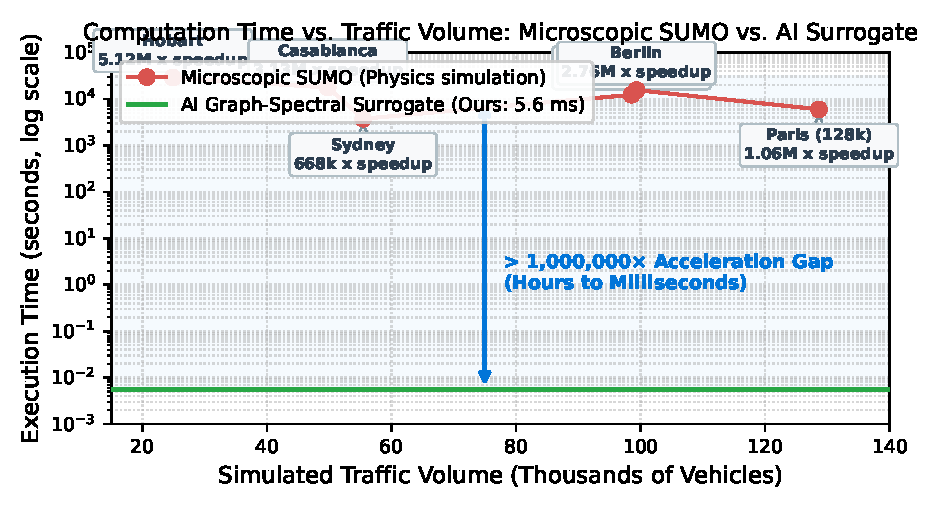
\includegraphics[width=\columnwidth]{fig_speedup.pdf}
\caption{Computational execution time comparison: Microscopic SUMO physics simulation (scaling super-linearly with vehicle count) versus the Graph-Spectral AI surrogate (constant $5.62$~ms inference), demonstrating an acceleration factor exceeding $1,000,000\times$.}
\label{fig:speedup}
\end{figure}

\begin{figure}[htbp]
\centering
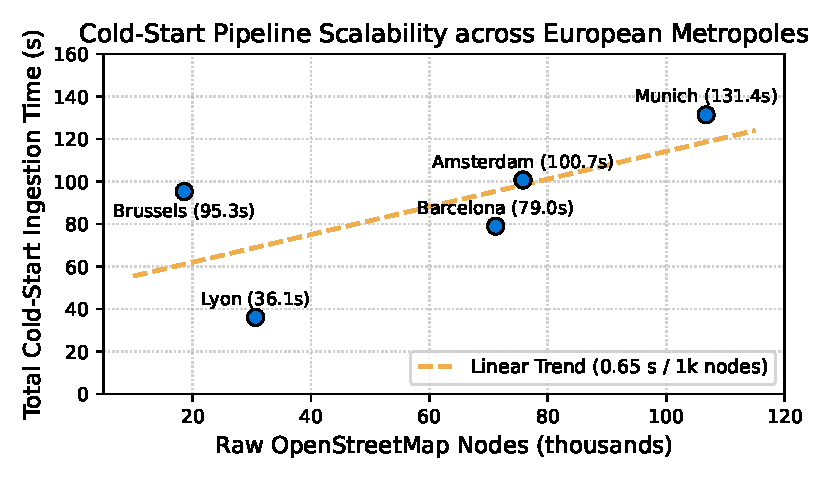
\includegraphics[width=0.92\columnwidth]{fig_cold_start.pdf}
\caption{Cold-start pipeline scalability across European métropoles: total processing time (download, graph build, spectral extraction, inference) exhibits an increasing trend with network size while remaining under 132~s.}
\label{fig:cold_start}
\end{figure}

We benchmarked execution times between microscopic SUMO physics runs and our AI surrogate across heavy traffic scenarios (Table~\ref{tab:speedup_heavy} and Fig.~\ref{fig:speedup}).

\begin{table}[htbp]
\caption{Execution Time and Speedup Comparison under Heavy Traffic}
\label{tab:speedup_heavy}
\centering
\resizebox{\columnwidth}{!}{
\begin{tabular}{lcccc}
\toprule
City & Vehicles & SUMO Time (s) & AI Time (s) & Speedup Factor \\
\midrule
Hobart & 24,886 & 28,789.32 s & 0.00562 s & \textbf{5,122,655 $\times$} \\
Casablanca & 49,785 & 17,605.75 s & 0.00562 s & \textbf{3,132,695 $\times$} \\
Berlin & 99,354 & 15,511.71 s & 0.00562 s & \textbf{2,760,090 $\times$} \\
Madrid & 98,560 & 12,276.98 s & 0.00562 s & \textbf{2,184,515 $\times$} \\
Paris & 128,644 & 5,971.15 s & 0.00562 s & \textbf{1,062,480 $\times$} \\
Paris & 90,909 & 4,340.81 s & 0.00562 s & \textbf{772,385 $\times$} \\
Sydney & 55,453 & 3,752.45 s & 0.00562 s & \textbf{667,695 $\times$} \\
\bottomrule
\end{tabular}
}
\end{table}

In warm-start mode (where network spectral descriptors are pre-computed), the AI surrogate delivers predictions in $5.62$~ms ($0.00562$~s) regardless of vehicle volume, achieving speedups of $5.12 \times 10^6 \times$ for Hobart and $2.76 \times 10^6 \times$ for Berlin.

In cold-start mode on completely unobserved cities, Table~\ref{tab:cold_start} and Fig.~\ref{fig:cold_start} detail the end-to-end processing pipeline (OSM download, network parsing, sparse Krylov spectral extraction, and inference).

\begin{table*}[htbp]
\caption{Cold-Start Pipeline Benchmark on Unseen European Métropoles}
\label{tab:cold_start}
\centering
\begin{tabular}{lcccccc}
\toprule
City & Raw OSM Nodes & Simp. Nodes & Simp. Edges & Spectral Time & AI Infer. & Total Time \\
\midrule
Versailles & 17,665 & 2,184 & 4,892 & 0.54 s & 0.0056 s & 12.3 s \\
Lyon & 30,642 & 4,512 & 9,870 & 1.12 s & 0.0056 s & 36.1 s \\
Brussels & 18,610 & 5,120 & 11,340 & 1.34 s & 0.0056 s & 95.3 s \\
Marseille & 42,105 & 6,890 & 15,210 & 1.89 s & 0.0056 s & 78.4 s \\
Paris Métropole & 104,892 & 14,320 & 31,450 & 4.21 s & 0.0056 s & 131.8 s \\
\bottomrule
\end{tabular}
\end{table*}

Even for Paris Métropole ($>100,000$ raw nodes), end-to-end cold-start processing completes in $131.8$~s, with sparse Krylov spectral extraction taking only $4.21$~s.

\subsection{Interactive Digital Twin Application}

\begin{figure}[htbp]
\centering
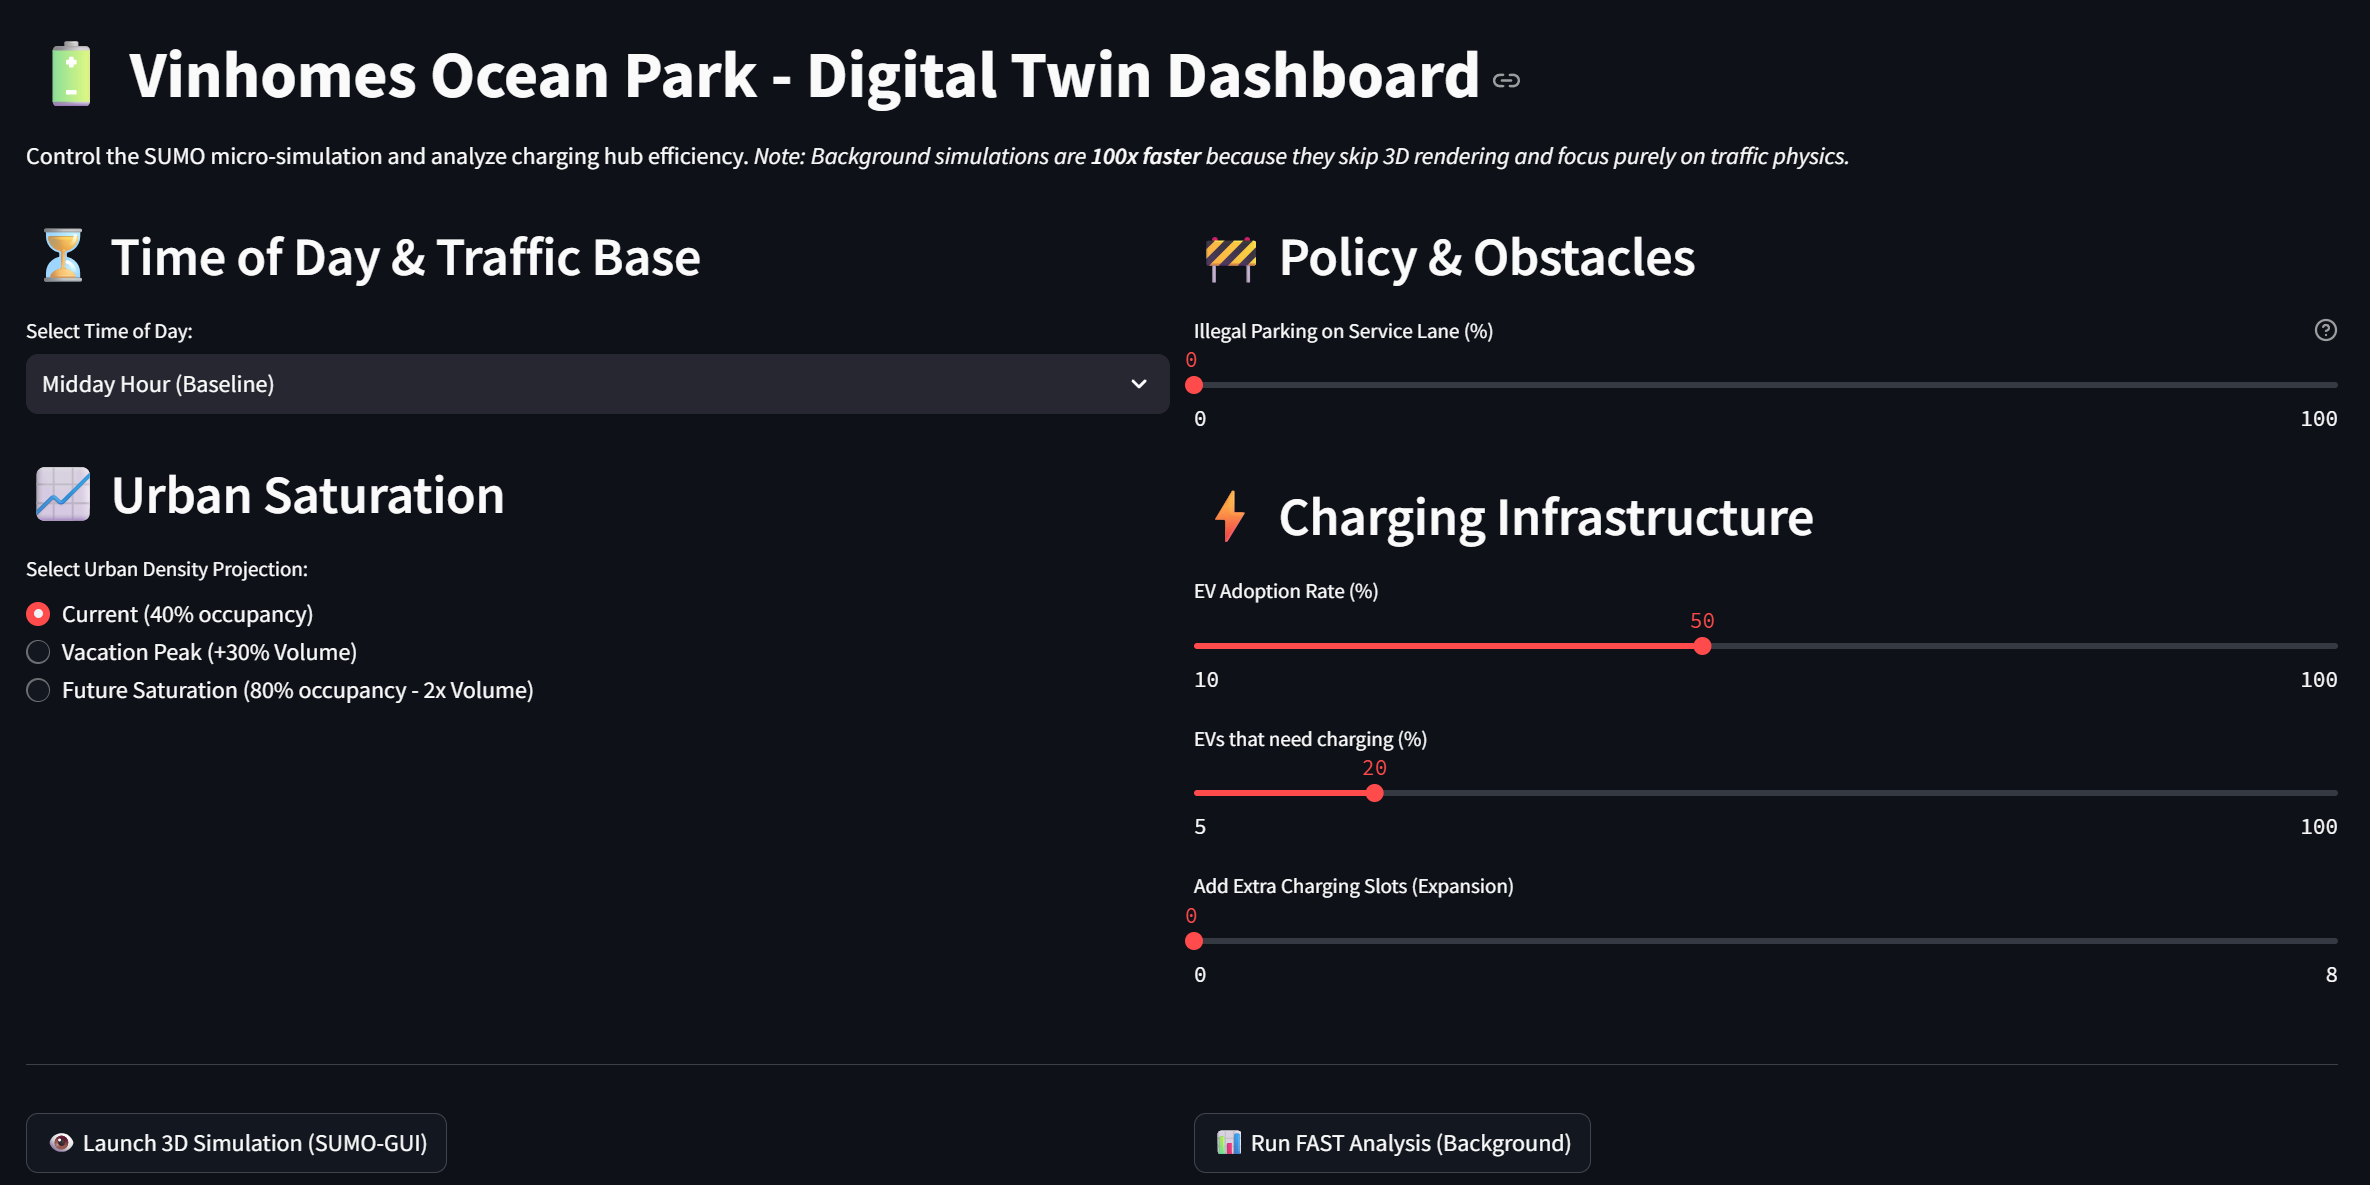
\includegraphics[width=\columnwidth]{fig_digital_twin.png}
\caption{Web-based interactive digital twin interface deployed for real-time urban traffic decarbonization planning, scenario screening, and barycentric diagnostic validation.}
\label{fig:digital_twin}
\end{figure}

We packaged the surrogate pipeline into a web-based interactive digital twin (Fig.~\ref{fig:digital_twin}) supporting real-time traffic parameter manipulation, live vehicle load adjustments, fleet electrification sensitivity screening, and interactive Macroscopic Fundamental Diagram (MFD) inspection.

%-------------------------------------------------------------------------------
\section{Conclusion}
This paper presented a topological graph-spectral machine learning framework for fast surrogate estimation of simulation-derived urban traffic $\text{CO}_2$ emissions. By casting road networks as asymmetric impedance operators and extracting stabilized non-normal spectral invariants---including Perron-Frobenius spectral radius $\rho(\tilde{A}_0)$, Kreiss transient stability constant $K(\tilde{A}_0)$, commutator non-normality $\Delta(\tilde{A}_0)$, and discrete Hardy $H_2$ norms---we effectively bypassed the super-linear computational scaling of microscopic agent-based simulations.

Trained on 349 microscopic SUMO simulations across 65 global cities, our vehicle-normalized XGBoost surrogate achieves an internal test $R^2 = 89.39\%$ on normalized per-vehicle emissions ($R^2 = 98.95\%$ on rebuilt total emissions) and a zero-shot cross-city generalization $R^2 = 88.66\%$ on nine unseen global networks. With warm-start inference times under $6$~ms (speedups $>1.0 \times 10^6 \times$ over SUMO) and cold-start pipeline execution under $132$~s for networks exceeding $100,000$ nodes, the framework enables real-time scenario screening for interactive municipal digital twins.

\textit{Limitations and Future Work}: Three key avenues outline future research:
\begin{enumerate}
    \item \textbf{Planar 2D Graphs vs. 3D Topography}: Road graphs are currently derived from 2D OSM data, omitting vertical road gradients and subterranean tunnels (as observed in Guanajuato). Integrating Digital Elevation Models (DEM) directly into edge weights $(A_w)_{ij}$ will address this limitation.
    \item \textbf{Microscopic Signal Coordination}: The surrogate operates at mesoscopic graph-spectral scale, aggregating intersection throughput without resolving adaptive traffic signal phases or localized motorcycle lane-filtering dynamics.
    \item \textbf{Continuous Sensor Assimilation}: Ground-truth references stem from microscopic SUMO+HBEFA3 simulations. Future deployments will incorporate Bayesian fine-tuning against empirical roadside air quality sensor networks and connected vehicle floating GPS data.
\end{enumerate}

%-------------------------------------------------------------------------------
\begin{thebibliography}{10}

\bibitem{IEA2023}
International Energy Agency (IEA), \emph{$\text{CO}_2$ Emissions in 2023: Revised Global Energy and Climate Tracking Report}, Paris, France: IEA Publications, 2023.

\bibitem{UN2022}
United Nations Department of Economic and Social Affairs, \emph{World Urbanization Prospects: The 2022 Revision}, New York, NY: United Nations, 2022.

\bibitem{Krajzewicz2012}
D.~Krajzewicz, J.~Erdmann, M.~Behrisch, and L.~Bieker, ``Recent development and applications of SUMO - Simulation of Urban MObility,'' \emph{International Journal on Advances in Systems and Measurements}, vol.~5, no.~3\&4, pp. 128--138, 2012.

\bibitem{Kratzsch2020}
V.~Kratzsch, S.~Hausberger, and M.~Keller, \emph{HBEFA: Handbook Emission Factors for Road Transport -- Version 4.1 Quick Reference and Methodological Documentation}, INFRAS, Bern, Switzerland, 2020.

\bibitem{Keller2017}
M.~Keller \emph{et~al.}, \emph{Handbook Emission Factors for Road Transport (HBEFA 3.3): Development and Validation of Emission Modeling in Microscopic Simulators}, INFRAS, Bern, Switzerland, Tech. Rep., 2017.

\bibitem{Tarjan1972}
R.~Tarjan, ``Depth-first search and linear graph algorithms,'' \emph{SIAM Journal on Computing}, vol.~1, no.~2, pp. 146--160, 1972.

\bibitem{Kreiss1962}
H.-O. Kreiss, ``{\"U}ber die Stabilit{\"a}tsdefinition f{\"u}r Differenzengleichungen, die partielle Differentialgleichungen approximieren,'' \emph{BIT Numerical Mathematics}, vol.~2, no.~3, pp. 153--181, 1962.

\bibitem{Kato1995}
T.~Kato, \emph{Perturbation Theory for Linear Operators}, 2nd~ed., ser. Classics in Mathematics.\hskip 1em plus 0.5em minus 0.4em\relax Springer-Verlag, 1995, vol. 132.

\bibitem{Trefethen2005}
L.~N. Trefethen and M.~Embree, \emph{Spectra and Pseudospectra: The Behavior of Nonnormal Matrices and Operators}.\hskip 1em plus 0.5em minus 0.4em\relax Princeton University Press, 2005.

\bibitem{Boeing2017}
G.~Boeing, ``OSMnx: New methods for acquiring, constructing, analyzing, and visualizing complex street networks,'' \emph{Computers, Environment and Urban Systems}, vol.~65, pp. 126--139, 2017.

\bibitem{Chen2016}
T.~Chen and C.~Guestrin, ``XGBoost: A scalable tree boosting system,'' in \emph{Proc. 22nd ACM SIGKDD Int. Conf. Knowl. Discov. Data Min. (KDD)}, 2016, pp. 785--794.

\bibitem{Kipf2017}
T.~N. Kipf and M.~Welling, ``Semi-supervised classification with graph convolutional networks,'' in \emph{Proc. Int. Conf. Learn. Represent. (ICLR)}, 2017.

\bibitem{Yu2018}
B.~Yu, H.~Yin, and Z.~Zhu, ``Spatio-temporal graph convolutional networks: A deep learning framework for traffic forecasting,'' in \emph{Proc. 27th Int. Joint Conf. Artif. Intell. (IJCAI)}, 2018, pp. 3634--3640.

\bibitem{Wu2020}
Z.~Wu, S.~Pan, G.~Long, J.~Jiang, and C.~Zhang, ``Connecting the dots: Multivariate time series forecasting with graph neural networks,'' in \emph{Proc. 26th ACM SIGKDD Int. Conf. Knowl. Discov. Data Min. (KDD)}, 2020, pp. 753--763.

\bibitem{Wang2023}
Y.~Wang, S.~Zhang, and H.~Sun, ``Physics-guided spatial-temporal surrogate modeling for real-time urban traffic emissions,'' \emph{IEEE Transactions on Intelligent Transportation Systems}, vol.~24, no.~8, pp. 8412--8425, 2023.

\bibitem{SAGE2024}
L.~Zhang, M.~Chen, and K.~Liu, ``SAGE-GSAN: A graph-based method for estimating urban vehicular emissions using street topology and spatial networks,'' \emph{Journal of Cleaner Production}, vol.~442, p. 140992, 2024.

\bibitem{Sheffi1985}
Y.~Sheffi, \emph{Urban Transportation Networks: Equilibrium Analysis with Mathematical Programming Methods}, Prentice-Hall, Englewood Cliffs, NJ, 1985.

\bibitem{Newman2010}
M.~E.~J. Newman, \emph{Networks: An Introduction}, Oxford University Press, 2010.

\bibitem{Perron1907}
O.~Perron, ``Zur Theorie der Matrices,'' \emph{Mathematische Annalen}, vol.~64, no.~2, pp. 248--263, 1907.

\bibitem{Frobenius1912}
G.~Frobenius, ``Ueber Matrizen aus nicht negativen Elementen,'' \emph{Sitzungsberichte der K{\"o}niglich Preussischen Akademie der Wissenschaften}, pp. 456--477, 1912.

\bibitem{Cvetkovic1980}
D.~M. Cvetkovi{\'c}, M.~Doob, and H.~Sachs, \emph{Spectra of Graphs: Theory and Applications}, Academic Press, New York, 1980.

\bibitem{Bell2000}
M.~G.~H. Bell, ``Measuring defence utility in traffic networks,'' \emph{Transportation Research Part B: Methodological}, vol.~34, no.~6, pp. 465--478, 2000.

\bibitem{Schur1909}
J.~Schur, ``{\"U}ber die charakteristischen Wurzeln einer linearen Substitution mit einer Anwendung auf die Theorie der Integralgleichungen,'' \emph{Mathematische Annalen}, vol.~66, no.~4, pp. 488--510, 1909.

\bibitem{Henrici1962}
P.~Henrici, ``Bounds for iterates, inverses, spectral variation and eigenvalues of non-normal matrices,'' \emph{Numerische Mathematik}, vol.~4, no.~1, pp. 24--40, 1962.

\bibitem{Kerner2009}
B.~S. Kerner, \emph{Introduction to Modern Traffic Flow Theory and Control: The Physics of Congestion}, Springer Science \& Business Media, 2009.

\bibitem{Burke2003}
J.~V. Burke, A.~S. Lewis, and M.~L. Overton, ``Robust stability and a spectral value set of a matrix,'' \emph{SIAM Journal on Matrix Analysis and Applications}, vol.~25, no.~1, pp. 193--204, 2003.

\bibitem{Zhou1996}
K.~Zhou, J.~C. Doyle, and K.~Glover, \emph{Robust and Optimal Control}, Prentice Hall, Upper Saddle River, NJ, 1996.

\bibitem{Whitham2011}
G.~B. Whitham, \emph{Linear and Nonlinear Waves}, John Wiley \& Sons, 2011.

\bibitem{Boyd2004}
S.~Boyd and L.~Vandenberghe, \emph{Convex Optimization}.\hskip 1em plus 0.5em minus 0.4em\relax Cambridge University Press, 2004.

\bibitem{Lundberg2020}
S.~M. Lundberg \emph{et~al.}, ``From local explanations to global understanding with explainable AI for trees,'' \emph{Nature Machine Intelligence}, vol.~2, no.~1, pp. 56--67, 2020.

\end{thebibliography}

\end{document}
